\section{Results}

\subsection{Correlation of Individual IQA Metrics with Human Perception}

The correlation analysis between individual FR-IQA metrics and human-rated MOS revealed substantial variability in performance. As shown in Fig.~\ref{fig:mos_vs_iqa}, several metrics exhibit strong linear trends with MOS, while others are poorly aligned or even negatively correlated. To quantify this, we ranked all 41 metrics based on the average of their PLCC and SRCC.\@

Fig.~\ref{fig:ranking} presents this ranking, highlighting that metrics such as PSNR, PSNR-B~\cite{ma2011psnr}, and MS-SSIM~\cite{wang2003multiscale} show the highest alignment with subjective opinion, while others, such as SRSIM~\cite{wang2004image}, diverge significantly.


\begin{figure}
    \centering
    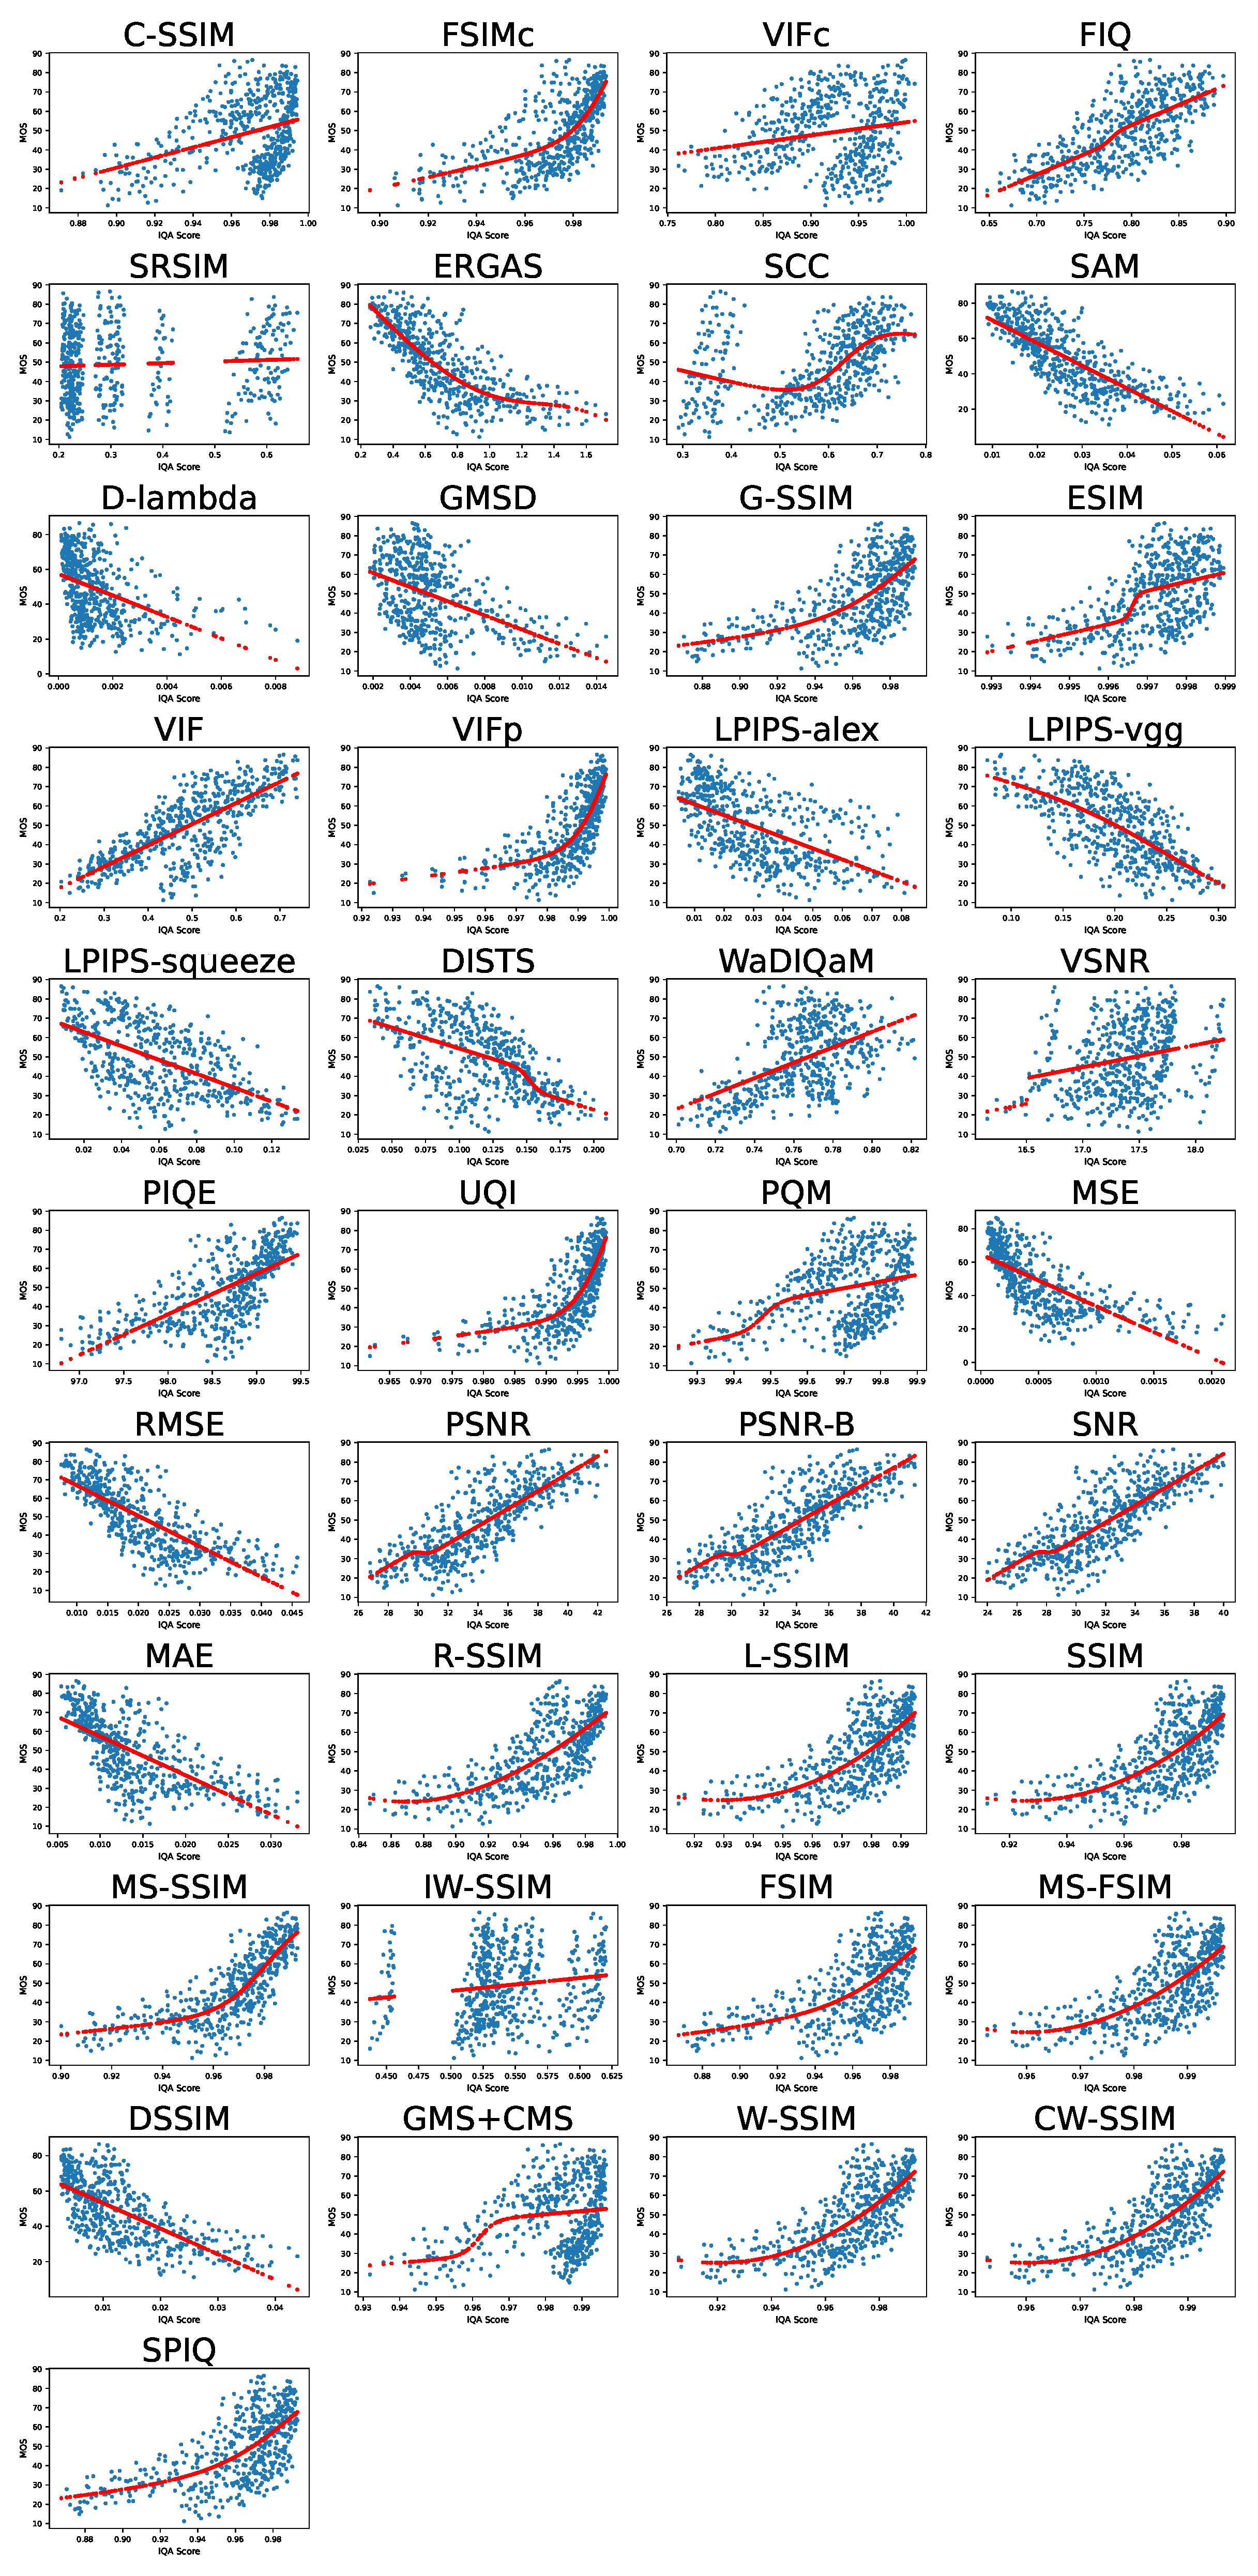
\includegraphics[width=0.7\linewidth]{images/mos_vs_iqa_grid.eps}
    \caption{Scatter plots illustrating the relationship between Mean Opinion Scores (MOS) and individual Full-Reference IQA metrics.}\label{fig:mos_vs_iqa}
\end{figure}

\begin{figure}
    \centering
    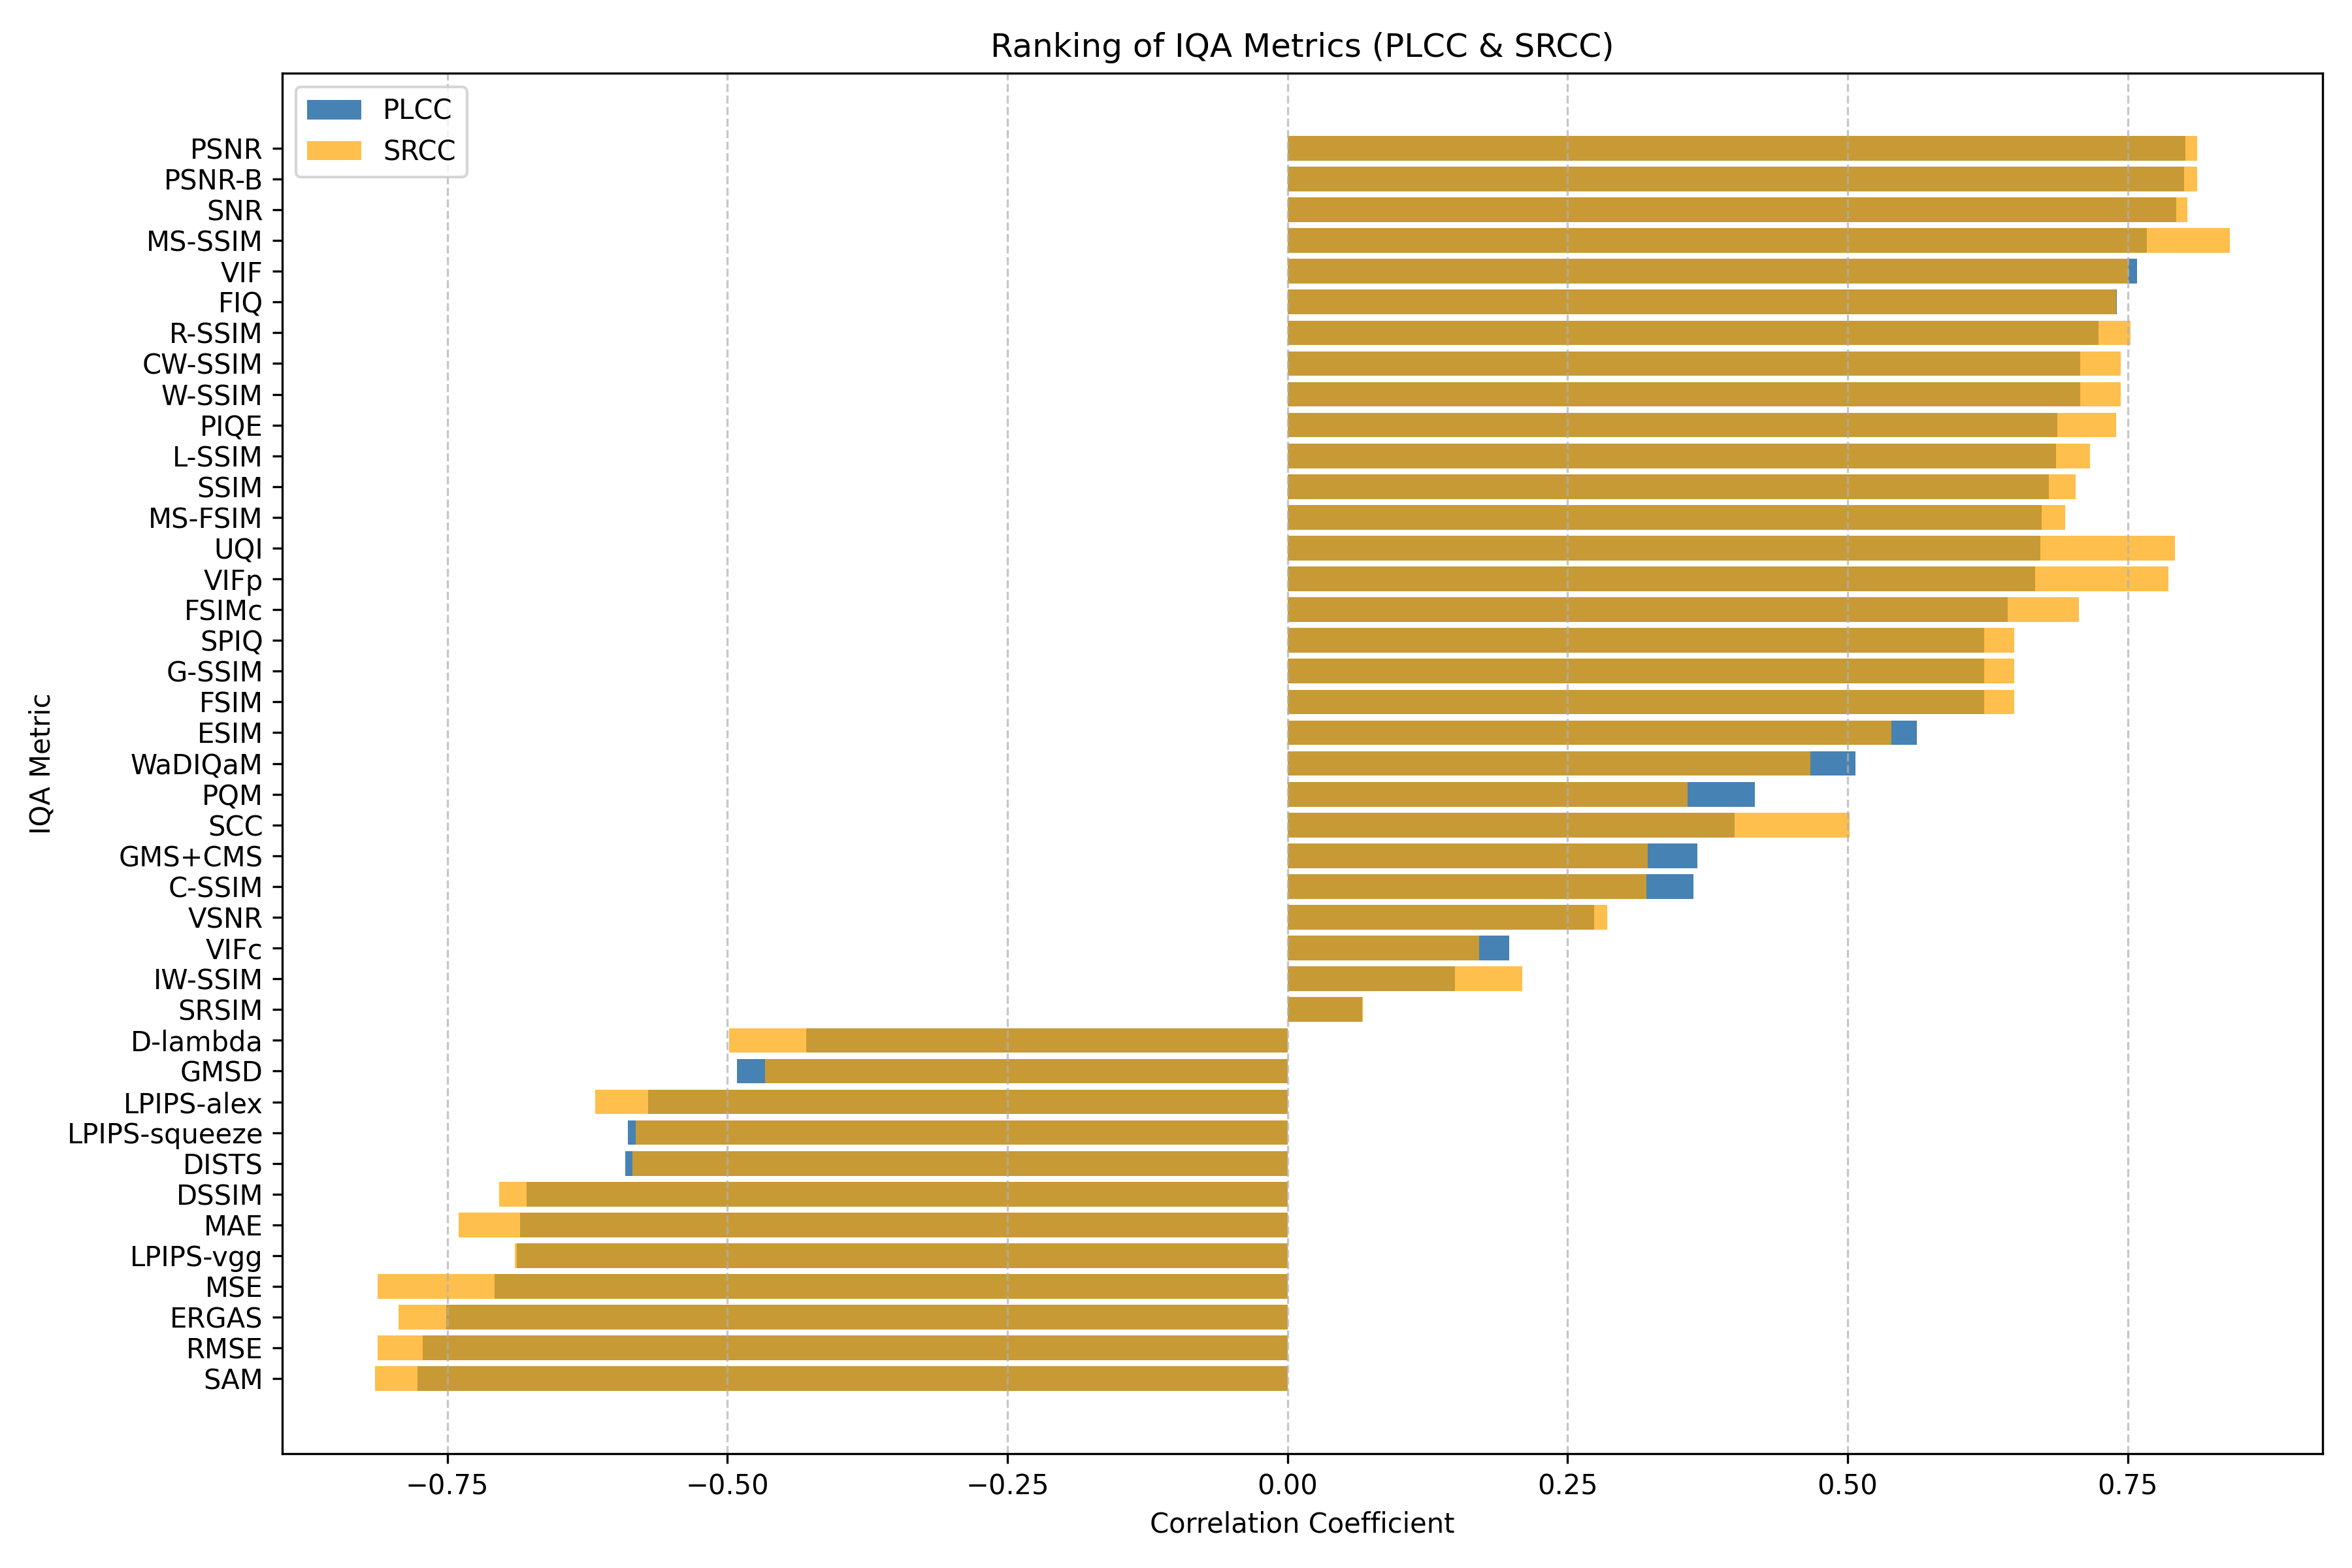
\includegraphics[width=0.9\linewidth]{images/metrics_bar.png}
    \caption{Ranking of FR-IQA metrics by correlation with MOS (PLCC and SRCC).}\label{fig:ranking}
\end{figure}

\subsection{Full-Reference Fusion Performance}

Using the 432 MOS-labeled images and $k = 5$ best metrics, we evaluated six fusion models.

As summarized in Table~\ref{tab:fusion_scores}, the Random Forest regressor achieved the best overall performance across all four evaluation metrics, as seen in Fig.~\ref{fig:randomforest}. Notably, it reached a PLCC of 0.8582 and SRCC of 0.8637, outperforming both linear and gradient boosting approaches.

\begin{figure}
    \centering
    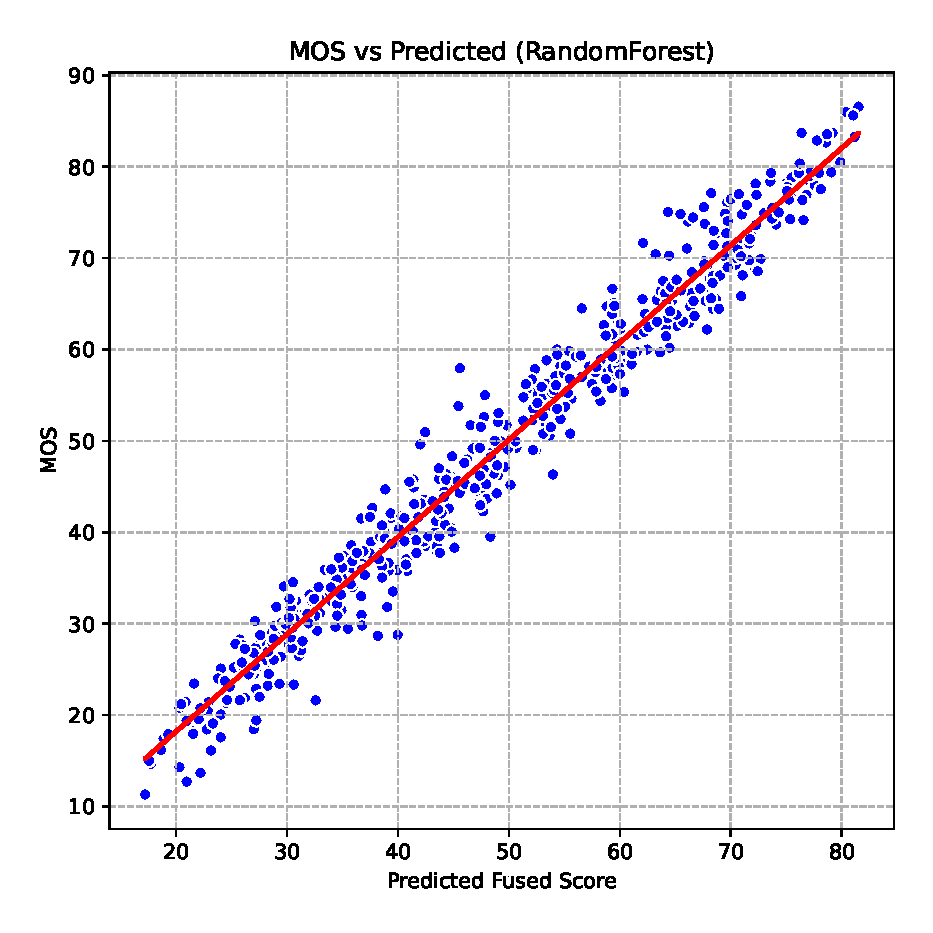
\includegraphics[width=0.6\linewidth]{images/fusion_plot_RandomForest.eps}
    \caption{MOS vs. Predicted fused Random Forest score}\label{fig:randomforest}
\end{figure}

\begin{table}
\caption{Fusion performance on 432 labeled images (MOS ground truth).}
\begin{center}
\begin{tabular}{lcccc}
\toprule
\textbf{Model} & \textbf{PLCC} & \textbf{SRCC} & \textbf{MSE} & \textbf{MAE} \\
\midrule
Linear Regression & 0.8123 & 0.8248 & 108.83 & 7.98 \\
Ridge             & 0.8125 & 0.8246 & 108.76 & 7.96 \\
Random Forest     & \textbf{0.8582} & \textbf{0.8637} & \textbf{84.48}  & \textbf{6.95} \\
SVR               & 0.8207 & 0.8207 & 108.44 & 8.08 \\
XGBoost           & 0.8560 & 0.8596 & 108.44 & 8.08 \\
LightGBM          & 0.8560 & 0.8577 & 85.90  & 7.15 \\
\bottomrule
\end{tabular}\label{tab:fusion_scores}
\end{center}
\end{table}

The trained Random Forest model was then applied to 3,132 unlabeled images, generating pseudo-MOS scores that serve as soft ground truth for the no-reference model.

\subsection{No-Reference Regression Model}

We trained a NR regressor using features extracted from a ResNet-18 pretrained on ImageNet. These features, paired with the pseudo-MOS scores generated from the fusion model, served as training data for a second Random Forest model.

Fig.~\ref{fig:nr_vs_fusion} shows the resulting alignment between the predicted NR quality scores and the fusion-based pseudo-MOS values. A clear linear trend is observed, with the model capturing both low and high quality regimes effectively.

\begin{figure}
    \centering
    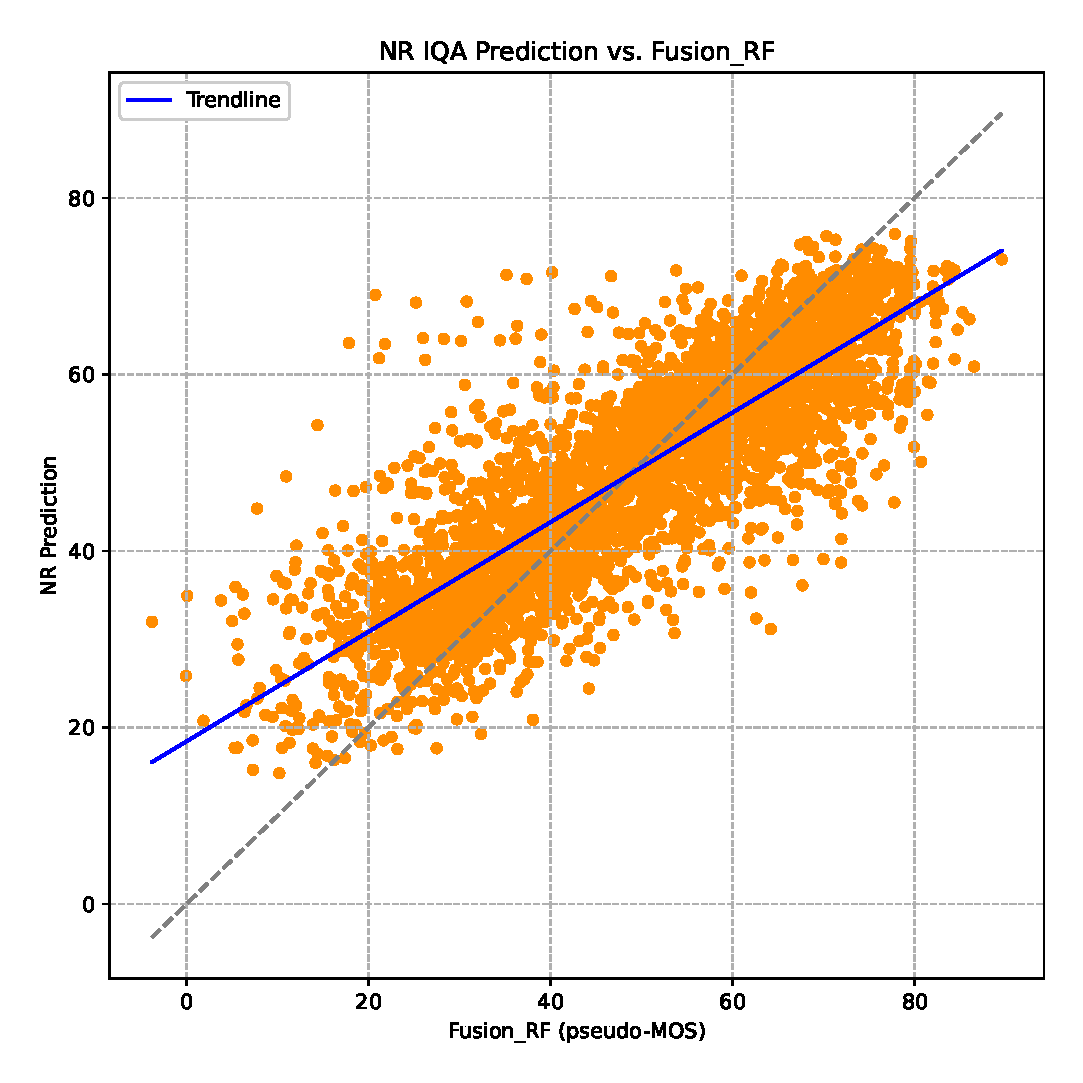
\includegraphics[width=0.6\linewidth]{images/nr_vs_fusion_rf.eps}
    \caption{Scatter plot of NR predictions vs.\ pseudo-MOS scores. The dashed line indicates identity; the blue line is the linear trend.}\label{fig:nr_vs_fusion}
\end{figure}

Quantitative results are reported in Table~\ref{tab:nr_scores}. Our proposed model, trained using deep features and pseudo-MOS supervision, achieves a PLCC of 0.8361 and SRCC of 0.8382, with an MSE of 90.48 and MAE of 7.16. In comparison, classical NR metrics such as NIQE and PIQE demonstrate weaker correlations with perceptual quality and substantially higher error. Even task-specific approaches like SER-FIQ and MagFace underperform, highlighting the robustness of our weakly supervised strategy for NR-IQA on steganographically degraded facial images.

\begin{table}
\caption{Performance of our NR IQA model, ResNet18 + Random Forest (RF), compared to standard NR-IQA baselines, using pseudo-MOS as ground truth.}
\begin{center}
\begin{tabular}{lcccc}
\toprule
\textbf{Method} & \textbf{PLCC} & \textbf{SRCC} & \textbf{MSE} & \textbf{MAE} \\
\midrule
Ours (ResNet18 + RF) & \textbf{0.8361} & \textbf{0.8382} & \textbf{90.48} & \textbf{7.16} \\
NIQE                 & 0.7536          & 0.7431          & 6859.81        & 82.62 \\
PIQE                 & 0.2993          & 0.3114          & 3297.65        & 57.05 \\
SER-FIQ              & -0.1648         & -0.1542         & 123.50         & 9.23 \\
MagFace              & -0.6095         & -0.6362         & 4437.91        & 66.24 \\
\bottomrule
\end{tabular}\label{tab:nr_scores}
\end{center}
\end{table}

